% !TEX root = ../main.tex
\chapter{Implementation of the Expansion Algorithm}

In this chapter we will explain the basic ideas on how to use the
expansion algorithm jointly with graph neural networks with the objective of generating terms
of a specific type in a given theory. We will also present a demo of the 
raw expansion algorithm for generating terms on simply typed combinatory logic
in order to give some intuition on how the algorithm works.

\section{Term generation in Simply Typed Combinatory Logic}

Now we will present the \textsc{implica} package for python \cite{fernandez}, a graph engine built on rust
rust that we built for the propose of this demonstration.
The idea of this package is to allocate the finite subcategory $G$,
and help to apply the different expansion iterations via its cypher-like interface
directly from python.

% TODO: cite Basic Proof Theory
First we will start by stating what simply typed Combinatory Logic, or $\textbf{CL}_\to$, is.
Given a countable set of type variables $P_0, P_1, P_2, \dots$, we define the set of simple types $\mathcal{T}_\to$ as
the set generated by the following clauses:
\begin{enumerate}
    \item type variables belong to $\mathcal{T}_\to$;
    \item if $A, B \in \mathcal{T}_\to$, then $(A \to B) \in \mathcal{T}_\to$.
\end{enumerate}
Types of the form $A \to B$ are called \textit{function types}, and are the simply
typed version of the product types we introduced in CoC.
Terms of $\textbf{CL}_\to$ must have a type assigned and are generated by the following clauses:
\begin{enumerate}
    \item for each $A \in \mathcal{T}_\to$ there is a countably infinite supply of variables of type $A$;
    \item if $t$, $s$ are terms of types $A \to B$ and $A$ respectively,
        then $\App(t, s)$ is a term of type $B$;
    \item for all $A, B, C \in \mathcal{T}_\to$ there are constant terms
        \[
          \clk^{A, B} \colon A \to B \to A
        \] \[
          \cls^{A, B, C} \colon (A \to B \to C) \to (A \to B) \to A \to C
        \]
\end{enumerate}
We will use the following notation: to assert that $t$ is a term of type $A$, we will write $t \colon A$;
instead of writing $\App(t, s)$ we can simply write $t s$. 
% TODO: add explanation on associativity of operations - parenthesis 

We can write this as a GAT signature as follows: 
\begin{align*} % TODO : fix overflow
    \vdash & \Prop \type \\
    p \colon \Prop \vdash & \Proof(p) \type \\
    A, B \colon \Prop \vdash & (A \to B) \colon \Prop \\
    A, B \colon \Prop, t \colon \Proof(A \to B), s \colon \Proof(A) \vdash  & \App(t, s) \colon \Proof(B) \\
    A, B \colon \Prop \vdash & \clk^{A, B} \colon \Proof(A \to B \to A) \\begin{align*}
    A, B, C \colon \Prop \vdash & \cls^{A, B, C} \colon \Proof((A \to B \to C) \to (A \to B) \to A \to C)
\end{align*}
This will let us leverage the construction of $C(U)$ we made for the general case, but this will be rather difficult
to follow. Hence, we will look for simplification both of the category and the expansion rules.
Consider $\Gamma$ a simple type expression of $\textbf{CL}_\to$, let $A_1, \dots, A_n$ be the type variables appearing on $\Gamma$,
and let $\Delta$ be the context $A_1 \colon \Prop, \dots, A_n \colon \Prop$. We center our search on the relativization of $C(U)$ by $\Delta$,
$\mathcal{C}_\Delta$. This is a contextual category, with all the tree structure, but this tree structure carries little-to-none meaning 
as we are working with "non-dependent" types, so by just considering objects of the first level and the final object we have all the 
possible types in $A_1, \dots, A_n$ and their relevant morphisms. Moreover, the object $[\Delta, x \colon \Prop]$ lies in the $\level$ $1$,
but it carries no important information in our case, as its just used for object formation by the general expansion algorithm, but 
that will be done differently in this special case, so we will remove it.
So we can consider $\mathcal{C}$ to be the full subcategory of $C(U)$ containing $[\Delta]$ and $[\Delta, x \colon \Proof(p)]$ for each term $p$
of type $\Prop$ under context $\Delta$.
The objects of this category are in 1-1-correspondence with the elements of $\mathcal{T}_\to \cup \{ 1 \}$, hence we will note \[
    1 \coloneqq [\Delta] \quad \text{ and } \quad  p \coloneqq [\Delta, x \colon \Proof(p)]
\]
In the case of morphisms, we will note them by the term appearing in the $n+1$ component, i.e. each morphism $\langle A_1, \dots, A_n, s \rangle$
in $\mathcal{C}$ will be noted as just $s$.
With this notation in mind we define the following rules of expansion: let $p$ be an element of $\mathcal{T}_\to$,
\begin{enumerate}
    \item if $p$ is of the form $B \to A$, we add \[
        A \xrightarrow{\clk^{A, B}} p
    \]
    \item for each $q$ in $G_n$ we add \[
        p \xrightarrow{\clk^{p, q}} q \to p
    \]
    \item if $p$ is of the form $(B \to A) \to A \to C$, we add \[
        (A \to B \to C) \xrightarrow{\cls^{A, B, C}} p
    \]
    \item if $p$ is of the form $(A \to B \to C)$, we add \[
        p \xrightarrow{\cls^{A, B, C}} ((A \to B) \to A \to C)
    \]
\end{enumerate}
Also, when creating an object $p$, if $p$ is of the form $A \to B \to A$, add the morphism $\clk^{A, B} \colon 1 \to p$, and if $p$ is of
the form $(A \to B \to C) \to (A \to B) \to A \to C$, add the morphism $\cls^{A, B, C} \colon 1 \to p$. Then, complete $G_{n+1}$ with the 
composition of morphisms in order for it to be a subcategory of $\mathcal{C}$.
The exhaustivity of this expansion algorithm is easy to check, as it follows directly from the definitions.

Now we will show how to code the expansion algorithm using python and the \textsc{implica} package. One peculiarity
we developed into \textsc{implica} that isn't part of our current definition is the fact that all terms of a type are 
considered equal, as we just care about having a witness, not the nature of it. In order to add this condition to the 
GAT signature, it's enough to add the following equation:
\[
    p \colon \Prop, t_1, t_2 \colon \Proof(p) \vdash t_1 = t_2
\]
But as it is not really part of combinatory logic we left it out of it's formal definition, but for our task it is 
more efficient to consider it this way.

First we will initialize an implica graph and we add the proposition $A \to A$ using the query API.
\begin{minted}{python}
    import implica

    graph = implica.Graph(
        constants = [
            implica.Constant(("K", "(A:*)->(B:*)->A")),
            implica.Constant("S", "((A:*)->(B:*)->(C:*))->(A->B)->A->C")
        ]
    )

    graph.query().create(f"(:{query})").execute()
\end{minted}

Now, to perform one expansion iteration we execute the following code
\begin{minted}{python}
    graph.query().match("(N:*)").set("N", { "existed" : True }).execute()

    (
        self.graph.query()
        .match("(N:(B:*) -> (A:*) { existed: true })")
        .create("(: A { existed: false })-[::@K(A, B)]->(N)")
        .execute()
    )
    (
        self.graph.query()
        .match("(N:(A:*) { existed: true })")
        .limit(10)
        .match("(M:(B:*) { existed: true })")
        .create("(N)-[::@K(A, B)]->(:B -> A { existed: false })")
        .execute()
    )
    (
        self.graph.query()
        .match("(N:((A:*) -> (B:*)) -> A -> (C:*) { existed: true })")
        .create("(:A->B->C { existed: false })-[::@S(A, B, C)]->(N)")
        .execute()
    )
    (
        self.graph.query()
        .match("(N:(A:*)->(B:*)->(C:*) { existed: true })")
        .create("(N)-[::@S(A, B, C)]->(:(A -> B) -> A -> C { existed: false })")
        .execute()
    )
\end{minted}
In the first line, we set an attribute "existed" to true in order to distinguish between new nodes and nodes already present at the beginning.
It is important to state the $.limit$ modifier on the second query, this is because this expansion rule creates, or tries to create
a new node for each pair of nodes in the graph, hence it makes complexity explode. To solve this we use the modifier $.limit$
to cap the number of creations per original node to $10$. Feel free to remove this line. 
This explosive growth of the complexity of the algorithm is what we will try to solve later by adding graph neural networks. 

Let's walk through, iteration by iteration, on the generation of a term of type $A \to A$ by the expansion algorithm to get some intuition. 
For simplicity, we have omitted the $1$ element on the graph displays, and also, as we just want witnesses of the existence of a term, we will just have at most one
morphism between two objects, and the sections (morphisms from $1$) will be displayed simply as red dots instead of blue.
The starting point $G_0$ is rather uninteresting as it just contains the object $A \to A$ with no section.
In the figure \ref{fig:g1-graph}, we can see $G_1$, it contains three unpopulated objects $A$, $A \to A$ and $(A \to A) \to A \to A$ from left to right.
Then, by applying another expansion we get $G_2$, figure \ref{fig:g2-graph}, where we start to see some objects getting populated, 
for example $(A \to A) \to A \to A$ with term $\cls \clk$. By the next expansion, $G_3$ grows significantly, see figure \ref{fig:g3-graph}, but $A \to A$ 
remains unpopulated. Finally, in $G_4$ $A \to A$ gets inhabited by the term $\cls \clk \clk$, but as you can see in figure \ref{fig:g4-graph}
the exponential growth of the graph continues.

\begin{figure}[htbp]
    \centering
    % First row
    \begin{subfigure}[b]{0.48\textwidth}
        \centering
        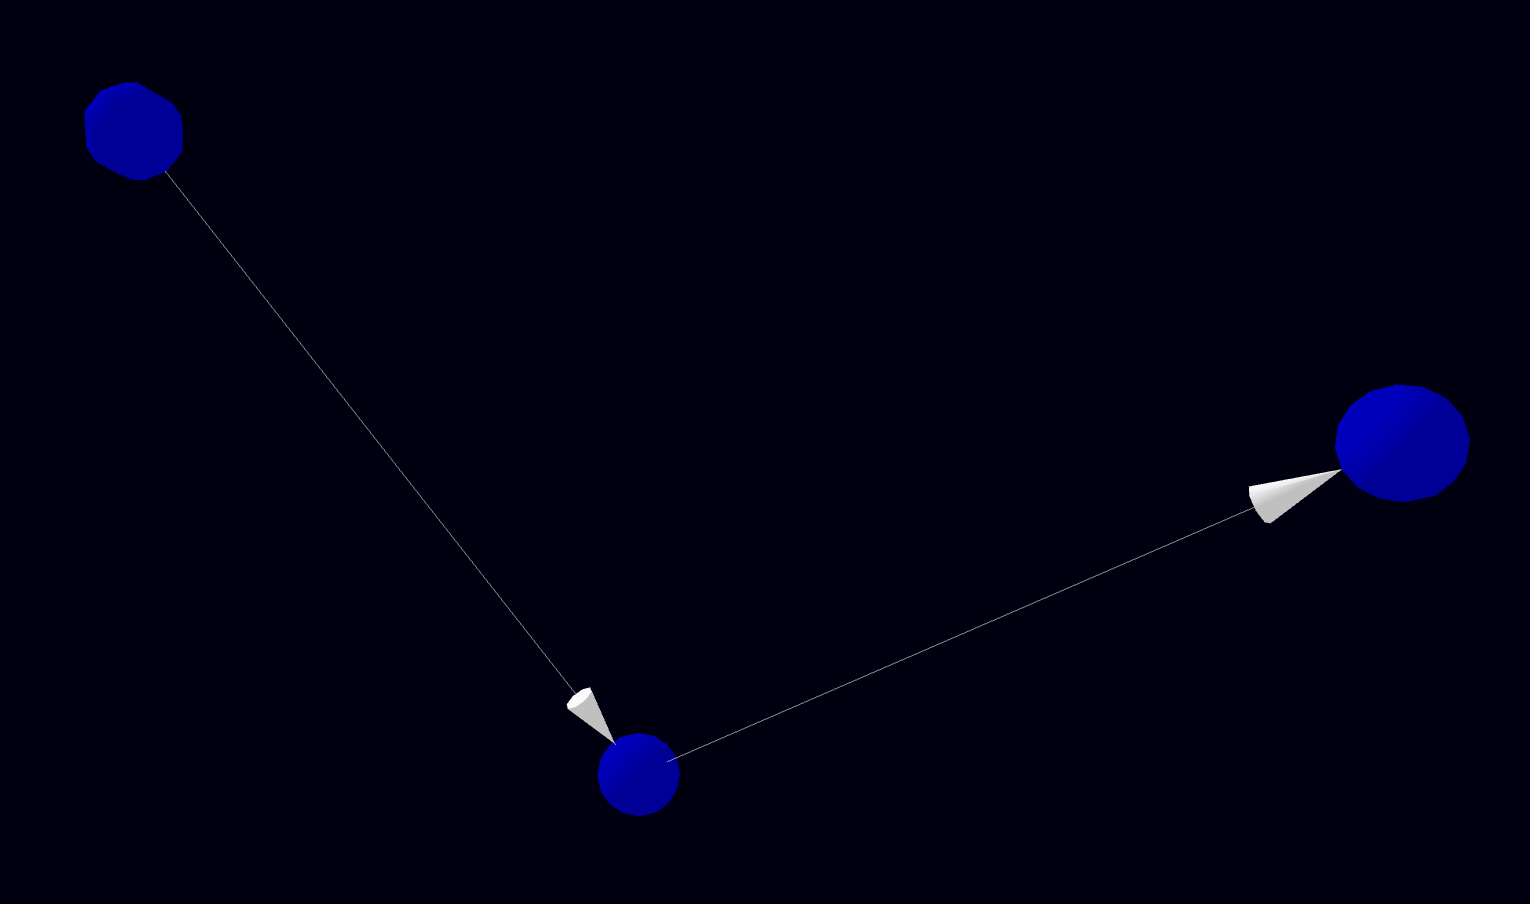
\includegraphics[width=\textwidth]{images/g1-graph.png}
        \caption{The $G_1$ subcategory}
        \label{fig:g1-graph}
    \end{subfigure}
    \hfill
    \begin{subfigure}[b]{0.48\textwidth}
        \centering
        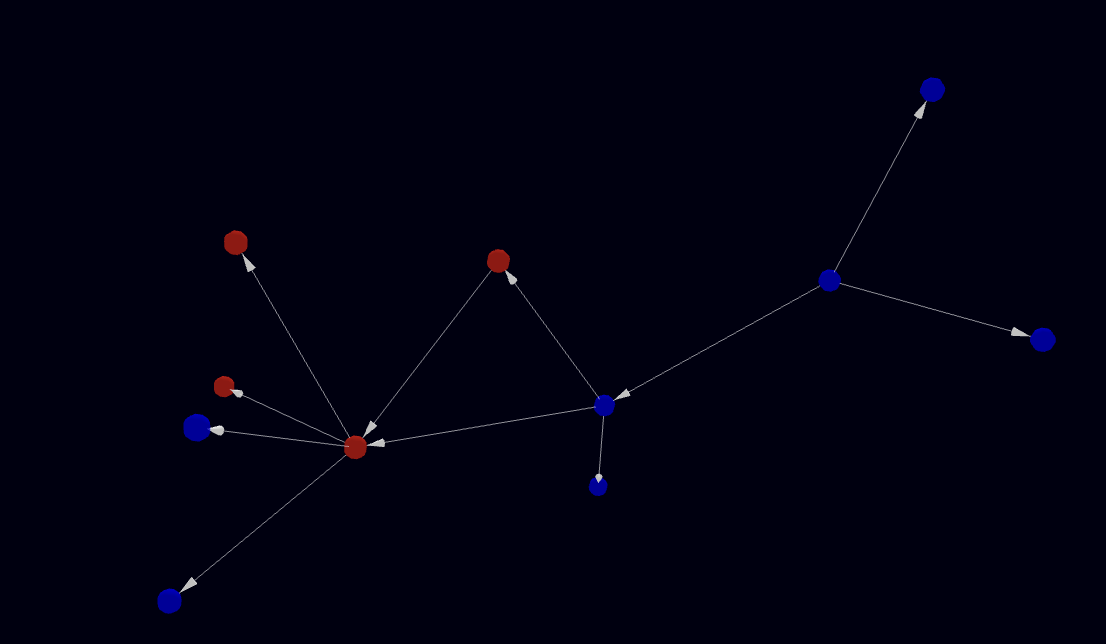
\includegraphics[width=\textwidth]{images/g2-graph.png}
        \caption{The $G_2$ subcategory}
        \label{fig:g2-graph}
    \end{subfigure}

    \vspace{1.5em} % Adds vertical space between the rows

    % Second row
    \begin{subfigure}[b]{0.48\textwidth}
        \centering
        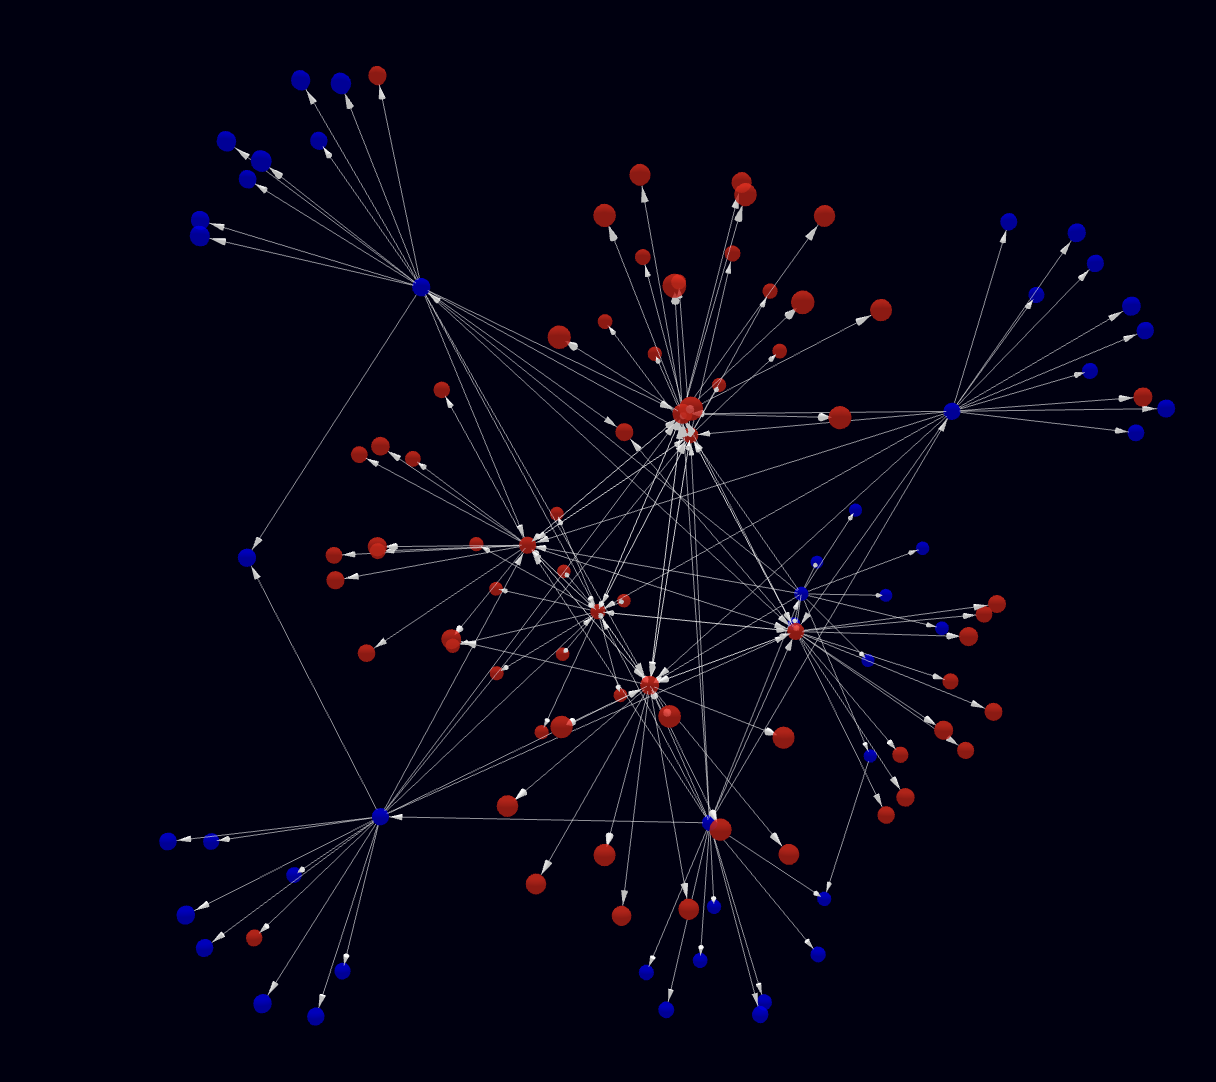
\includegraphics[width=\textwidth]{images/g3-graph.png}
        \caption{The $G_3$ subcategory}
        \label{fig:g3-graph}
    \end{subfigure}
    \hfill
    \begin{subfigure}[b]{0.48\textwidth}
        \centering
        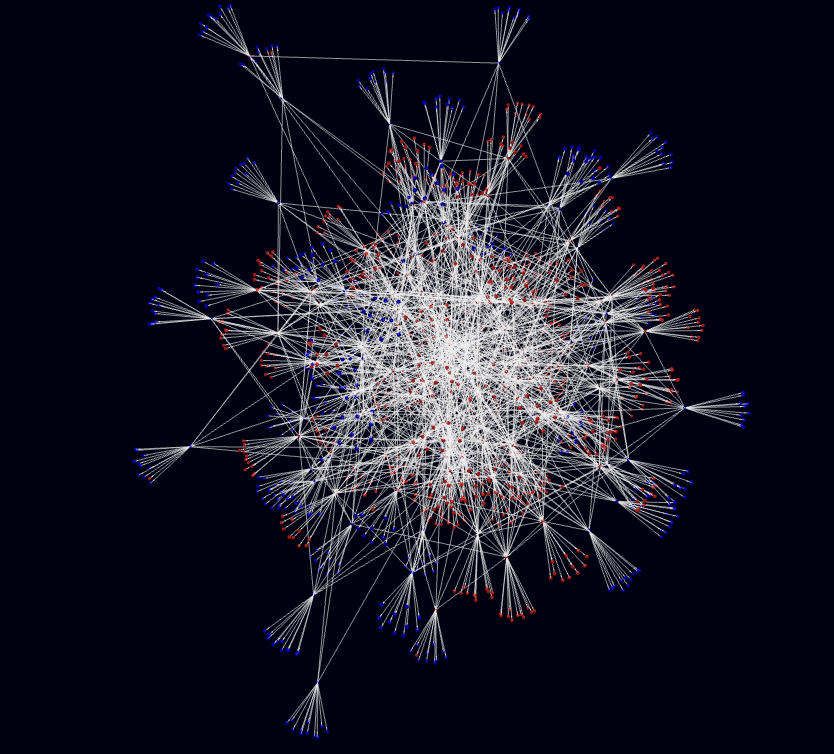
\includegraphics[width=\textwidth]{images/g4-graph.png}
        \caption{The $G_4$ subcategory}
        \label{fig:g4-graph}
    \end{subfigure}

    \caption{Overview of the $G_1$ through $G_4$ subcategories.}
    \label{fig:g-grid}
\end{figure}